\begin{chapter}{Описание модели. Кластерные режимы}
	\section{Модель Курамото с инерцией}
	В данной работе исследуется модель глобально связанных осцилляторов Курамото второго порядка, описываемая системой уравнений:
	\begin{equation} \label{main-sistem}
		m\ddot{\varphi}_i + \dot{\varphi}_i = \omega + 
		\frac{1}{N} \sum_{j = 1}^N \sin{(\varphi_j - 
		\varphi_i - \alpha)}, i = \overline{1, N}, 
	\end{equation}
	где $m$ -- параметр инерции, $\omega$ -- постоянный вращающий момент,
	$\alpha$ -- фазовая задержка, $N$ -- общее число элементов.
	Предполагается, что осцилляторы являются идентичными, с частотой $\omega$, массой $m$ и запаздыванием по
	фазе $\alpha \in [0, \pi)$ \cite{Sakaguchi} . В системе \eqref{main-sistem} имеется синфазный режим,
	который локально устойчив для любого $\alpha \in [0, \pi/2)$
	и неустойчив для любого $\alpha \in [\pi/2, \pi)$ \cite{Acebron:Bonilla}. Поэтому принято считать связь притягивающей при
	$\alpha < \pi/2$ и отталкивающей при $\pi/2 \leq \alpha < \pi$.

	\section{Двухкластерные вращательные режимы}
	
	Двухкластерный режим в модели \eqref{main-sistem} описывается системой:
	
	\begin{equation} \label{two-cluster}
		\begin{cases}
			m\ddot{\psi}_1 + \dot{\psi}_1 = \omega + \frac{N-K}{N} \sin{(\psi_2 - \psi_1 - \alpha)} - \frac{K}{N}\sin{\alpha},\\
			m\ddot{\psi}_2 + \dot{\psi}_2 = \omega + \frac{K}{N} \sin{(\psi_1 - \psi_2 - \alpha)} - \frac{N - K}{N}\sin{\alpha},
		\end{cases}
	\end{equation}
	где $\psi_1$, $\psi_2$ -- фазы элементов первого и
	второго кластера, соответственно, $K$ -- количество элементов в малом кластере.
	Введем новую переменную $\beta = \frac{K}{N}$, характеризующую долю элементов малого кластера относительно размера $N$ всего ансамбля.
	Уравнение \eqref{two-cluster} перепишется в виде:
	
	\begin{equation} \label{two-cluster-beta}
		\begin{cases}
			m\ddot{\psi}_1 + \dot{\psi}_1 = \omega + (1 - \beta) \sin{(\psi_2 - \psi_1 - \alpha)} - \beta\sin{\alpha}, \\
			m\ddot{\psi}_2 + \dot{\psi}_2 = \omega + \beta \sin{(\psi_1 - \psi_2 - \alpha)} - (1 - \beta)\sin{\alpha}.
		\end{cases}
	\end{equation}
	
	Введем величину $X = \psi_1 - \psi_2$, характеризующую расстройку фаз между элементами двух кластеров.
	Вычитая в \eqref{two-cluster-beta} из первого уравнения второе, приходим к уравнению для отстройки $X$:

	\begin{equation} \label{pre-pend}
		m\ddot{X} + \dot{X} = (1 - 2 \beta) \sin{\alpha} - \left[(1-\beta)\sin{(X + \alpha)} + \beta\sin{(X - \alpha)} \right].
	\end{equation}
	
	Заметим, что решение $X = 0$ соответствует реализации
	синфазного вращательного режима. Ненулевое решение $X \neq 0$ соответствует
	реализации двухкластерного режима.
	
	
	Для дальнейшего анализа уравнения \eqref{pre-pend} произведем ряд замен, а именно:
	\begin{align*}
	R^2 = (N - 2K)^2 \sin{\alpha}^2 + N^2 \cos{\alpha}^2, \\
	\rho = \sqrt{\frac{N}{m R}}, \ t = \hat{t} \frac{N}{\rho R}, \gamma = \frac{N - 2K}{R}\sin{\alpha}, \\
	\Phi = X + \delta, \ \delta = \arccos{(\frac{N}{R}\cos{\alpha})}, \\
	\end{align*}
	что приводит к:
	
	\begin{equation} \label{pend}
		\frac{d^2 \Phi }{d\hat{t}^2} + \rho \frac{d\Phi}{d\hat{t}} + \sin{\Phi} = \gamma.
	\end{equation}

	\begin{figure}[h!]
		\begin{center}
			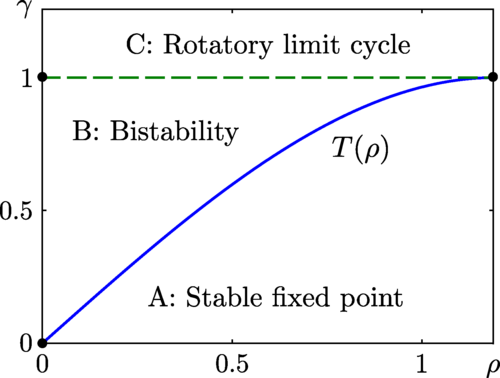
\includegraphics[width=0.7\columnwidth]{pictures/bf-tricommy.png}
		\end{center}
		\caption{Бифуркационная диаграмма маятникового уравнения \eqref{pend}}
		\label{bf-d}
	\end{figure}

	Полученное уравнение \eqref{pend} хорошо изучено в работе \cite{Andronov:Vitt}.
	В зависимости от параметров $\rho$ и $\gamma$, в системе \eqref{pend}
	могут существовать два состояния равновесия:
	устойчивая точка $\Phi_e = \arcsin{\gamma}$ и седло
	$\Phi_s = \pi - \arcsin{\gamma}$, а также
	некоторое устойчивое периодическое вращательное движение.
	Кривая $\gamma=T(\rho)$ называется кривой Трикоми и определяет границу области существования вращательного движения (области B и C).
	% Данные соотношения определяются так называемой
	% бифуркационной кривой Трикомми (см. рис. \ref{bf-d}).
	Таким образом, в исходной системе могут существовать 2 типа
	двухкластерных вращательных режимов, первый характеризуется
	постоянной расстройкой фаз, второй характеризуется
    периодической на цилиндре расстройкой фаз.
	Область существования вращательного движения в уравнении \eqref{pend}
	определяется соотношением:
	\begin{equation}
		\gamma \ge T(\rho),
		\label{eroi}
	\end{equation}
	где $T(.)$ -- уравнение кривой Трикоми. В качестве аппроксимации для кривой Трикоми можно использовать выражение
	$T(\rho) = \rho\frac{4}{\pi} - 0.305\rho^3$, полученное в \cite{Belykh:Brister}.
	Подставляя данную аппроксимацию кривой Трикому в уравнение \eqref{eroi} получаем уравнения для границы области существования двухкластерного вращательного движения с
	периодической расстройкой фаз в области параметров $\alpha$, $m$:
	\begin{equation} \label{borders}
		m = \frac{1}{\sqrt{(1 - 2\beta)^2\sin{\alpha}^2 + \cos{\alpha}^2} \cdot T^{-1}(\frac{(1 - 2\beta)\sin{\alpha}}{\sqrt{(1 - 2\beta)^2\sin{\alpha}^2 + \cos{\alpha}^2}})}.
	\end{equation}

	Заметим, что двухкластерный вращательный режим при $\beta = 0.5$ не существует.

	\begin{figure}[h!]
		\begin{center}
			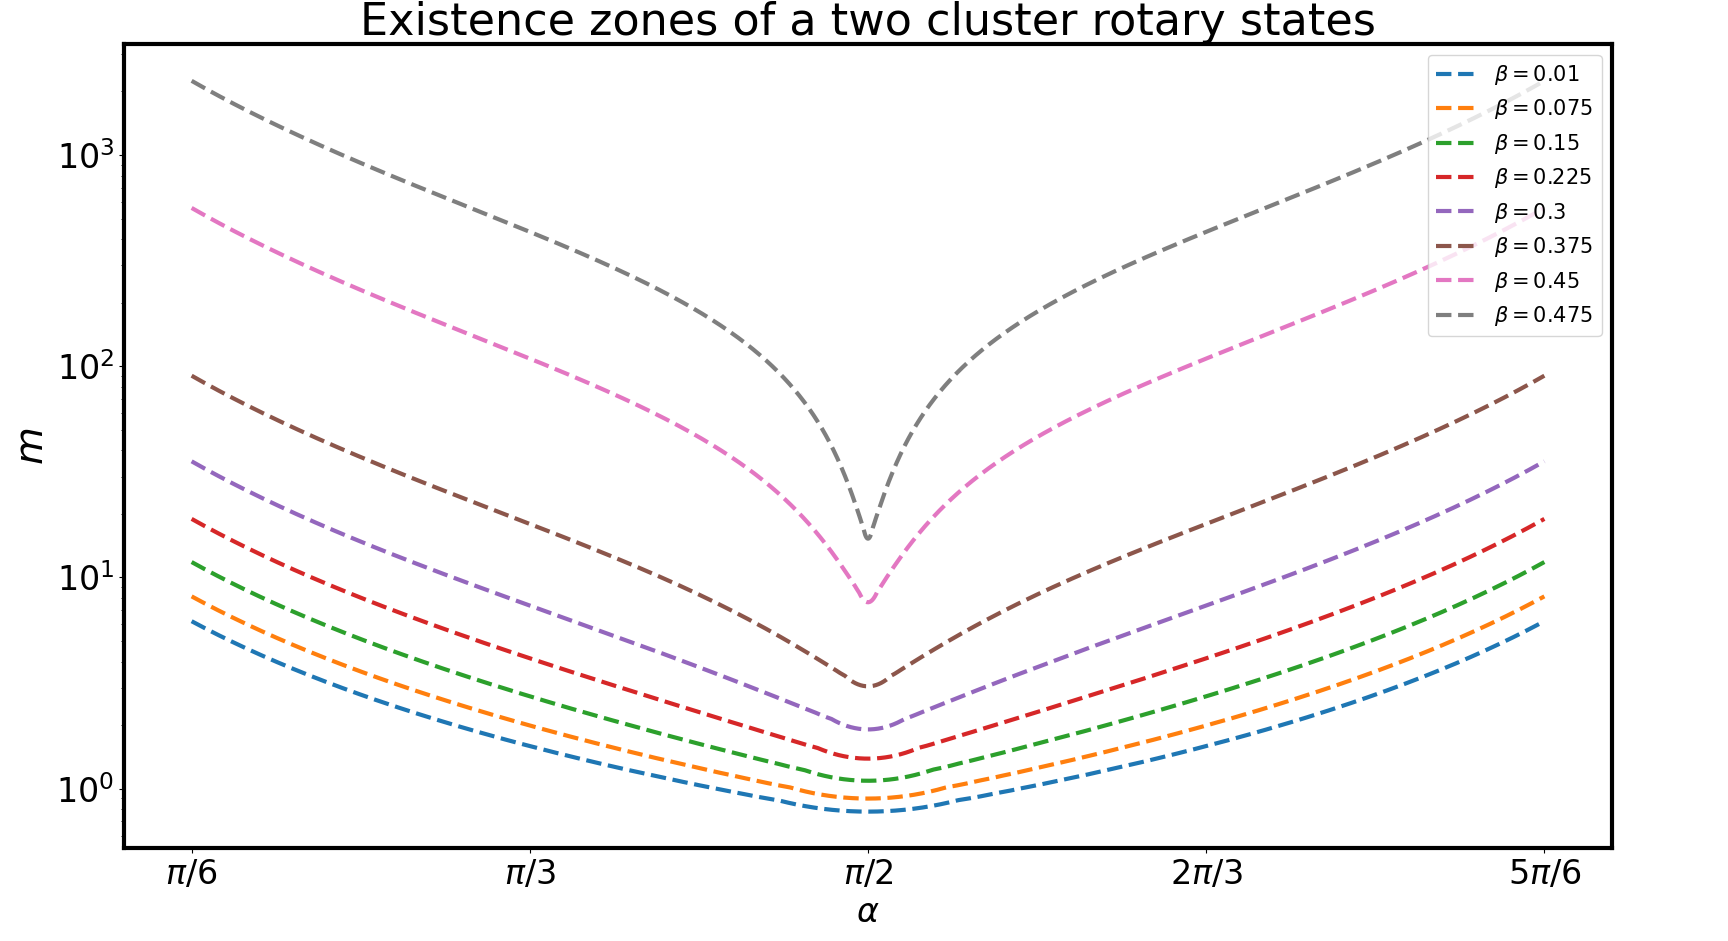
\includegraphics[width=1\columnwidth]{pictures/ex.png}
		\end{center}
		\caption{Границы зон устойчивости двухкластерного вращательного режима с вращающейся расстройкой фаз в зависимости от параметра $\beta$}
		\label{ex-zones}
	\end{figure}

	На рисунке \ref{ex-zones} изображены границы зон устойчивости двухкластерного вращательного режима
	с вращающейся расстройкой фаз в зависимости от параметра $\beta$.
	Можно заметить, что при фиксированном $N$ зона существования двухкластерного режима при размере малого кластера равного $K_1$ полностью включена в 
	зону существования двухкластерного режима при размере малого кластера равного $K_2$ при $K_1 > K_2$. Наблюдается мультистабильность вращательных режимов.


	На рисунке \ref{schema} изображены двухкластерные вращательные режимы в зависимости от параметра $N$.
	Каждая ячейка представляет собой определенный двухкластерный режим,
	характеризующийся параметром $\beta$, который записан в виде дроби в центре ячейки. Ячейки с одинаковым цветом, кроме серого, представляют собой
	один и тот же двухкластерный вращательный режим. Несложно заметить, что при фиксированном $N = N^*$
	двухкластерный вращательный режим, соответствующий $\beta^* = A/B$, где $A/B$ -- некоторая дробь,
	будет повторяться для всех $N = N^* + k\cdot B$. 

	\begin{figure}[h!]
		\begin{center}
			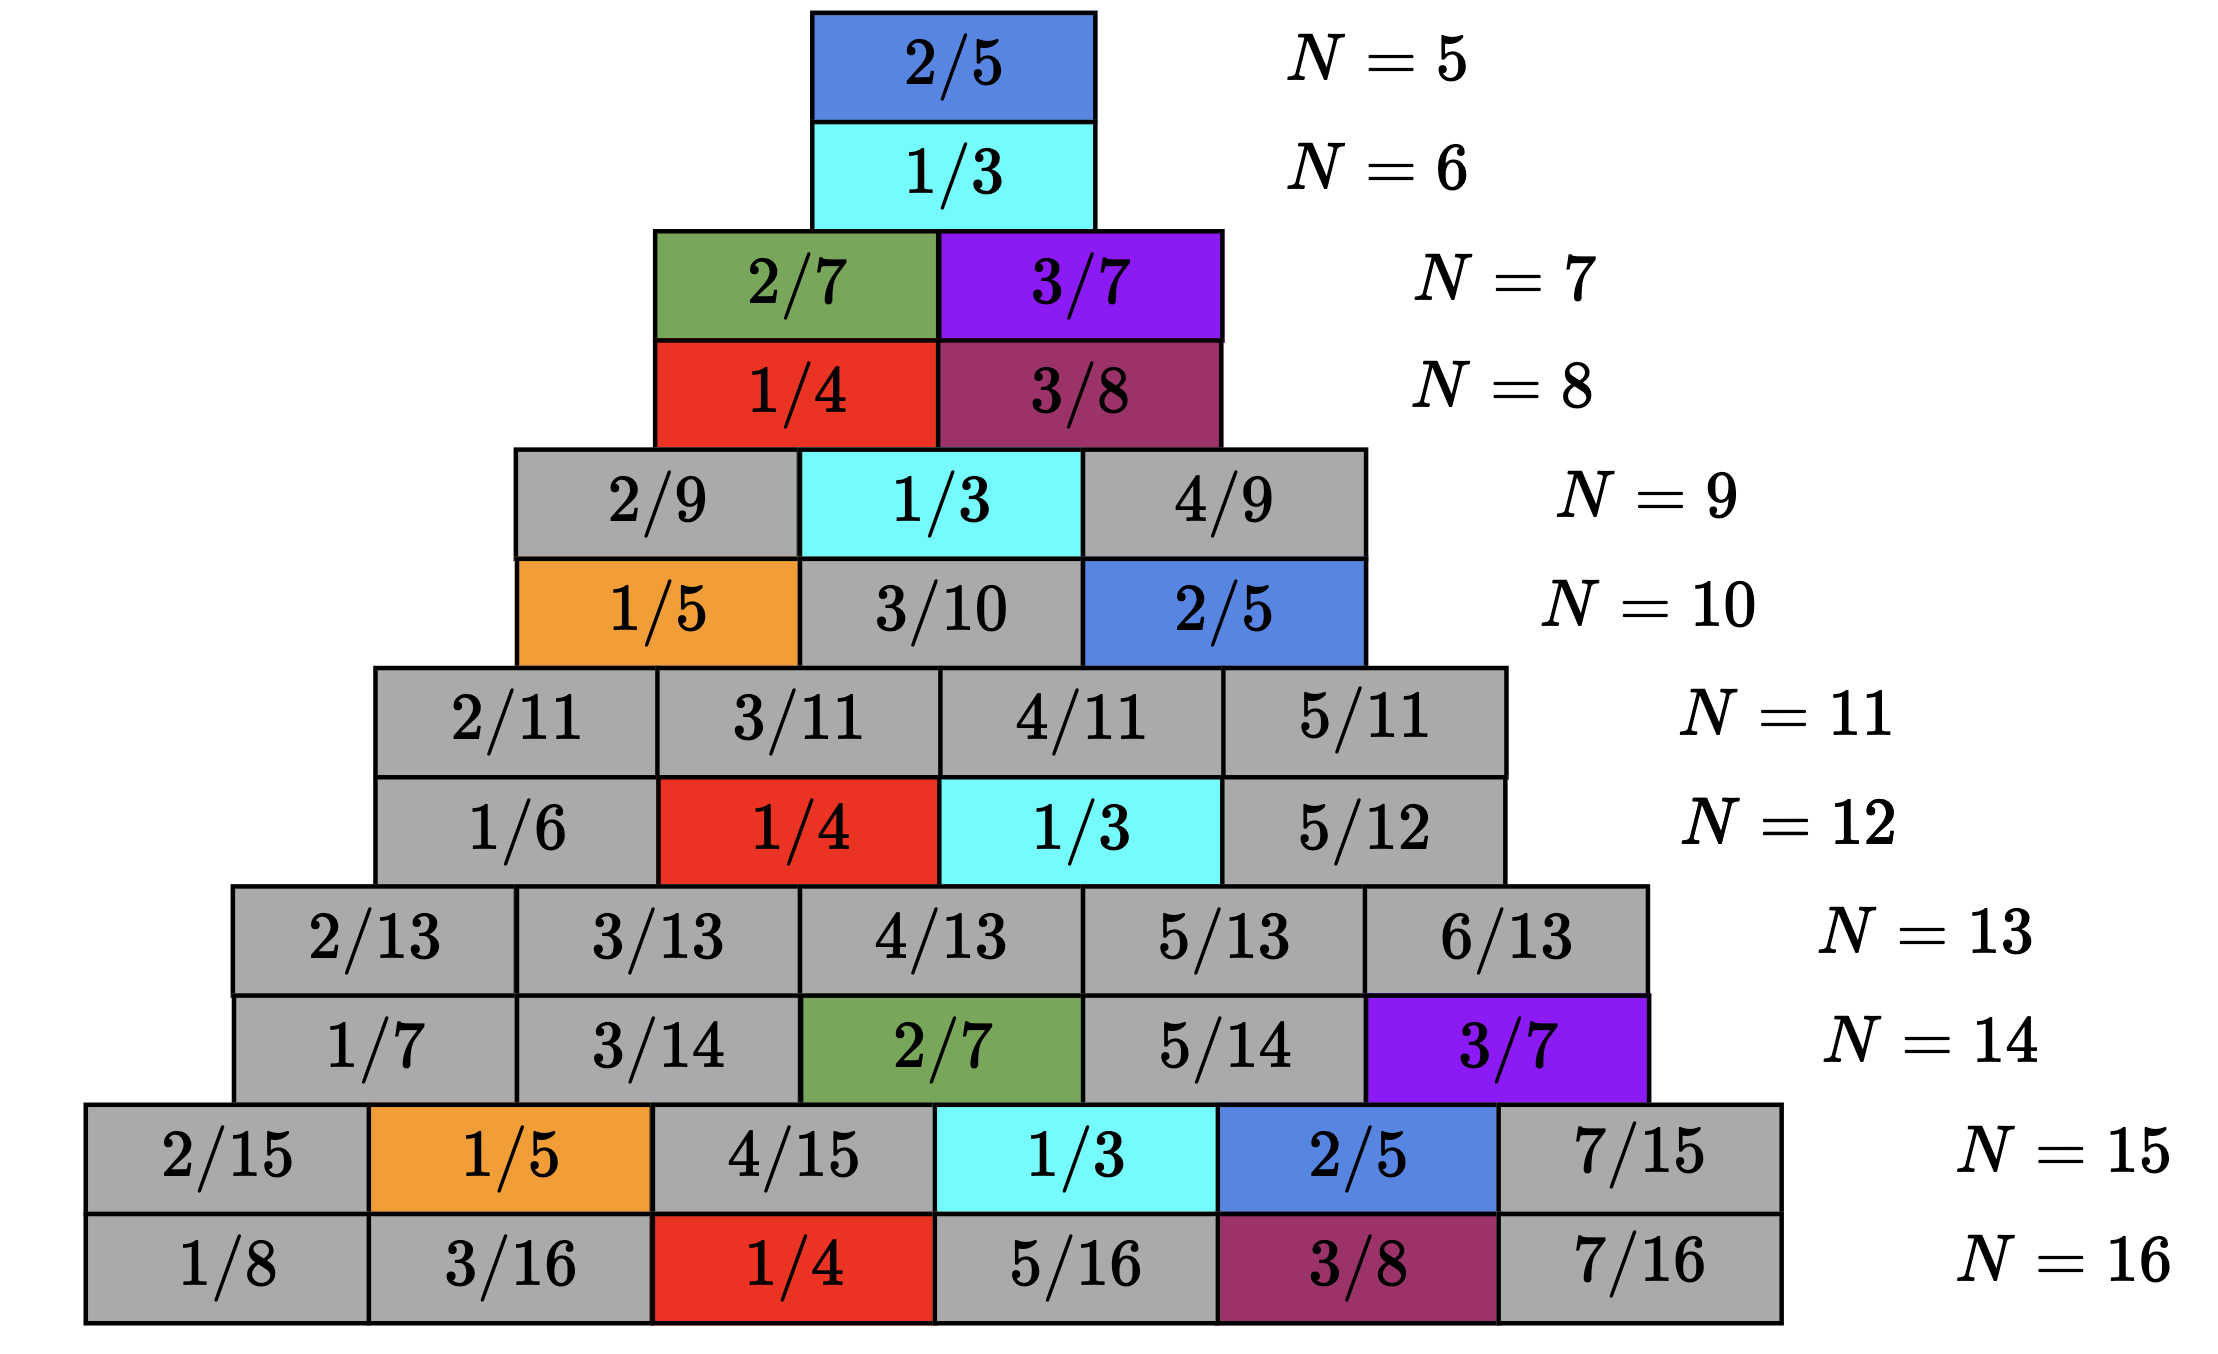
\includegraphics[width=1\columnwidth]{pictures/schema.png}
		\end{center}
		\caption{Двухкластерные вращательные режимы в зависимости от параметра $N$. Каждая ячейка представляет собой определенный двухкластерный режим,
		характеризующийся параметром $\beta$, который записан в виде дроби в центре ячейки. Ячейки с одинаковым цветом, кроме серого, представляют собой
		один и тот же двухкластерный вращательный режим}
		\label{schema}
	\end{figure}

\end{chapter}